%!TEX root = Report.tex
\chapter{Resultate und Diskussion}\label{sec:results}

Die Messergebnisse zeigen deutlich, dass die berechnete Gastemperatur ($T_{gas}$) weit unter den gemessenen Temperaturen $T_1$ und $T_2$ liegt und somit $\dot Q_{conv}$ stets negativ ist. $\dot Q_{conv} < 0$ bedeutet das Gas nimmt Wärme von der Lanze, bzw. diese wird vom Gas gekühlt.\\
Generell ist es offensichtlich, dass  Temperaturen eine  Verfälschung zwischen gemessenem und berechneten Wert aufweisen.

Lorem ipsum dolor sit amet, consectetuer adipiscing elit. Morbi commodo, ipsum sed pharetra gravida, orci magna rhoncus neque, id pulvinar odio lorem non turpis. Nullam sit amet enim. Suspendisse id velit vitae ligula volutpat condimentum. Aliquam erat volutpat. Sed quis velit. Nulla facilisi. Nulla libero. Vivamus pharetra posuere sapien. 

Nam consectetuer. Sed aliquam, nunc eget euismod ullamcorper, lectus nunc ullamcorper orci, fermentum bibendum enim nibh eget ipsum. Donec porttitor ligula eu dolor. Maecenas vitae nulla consequat libero cursus venenatis. Nam magna enim, accumsan eu, blandit sed, blandit a, eros.

\begin{figure}[H]
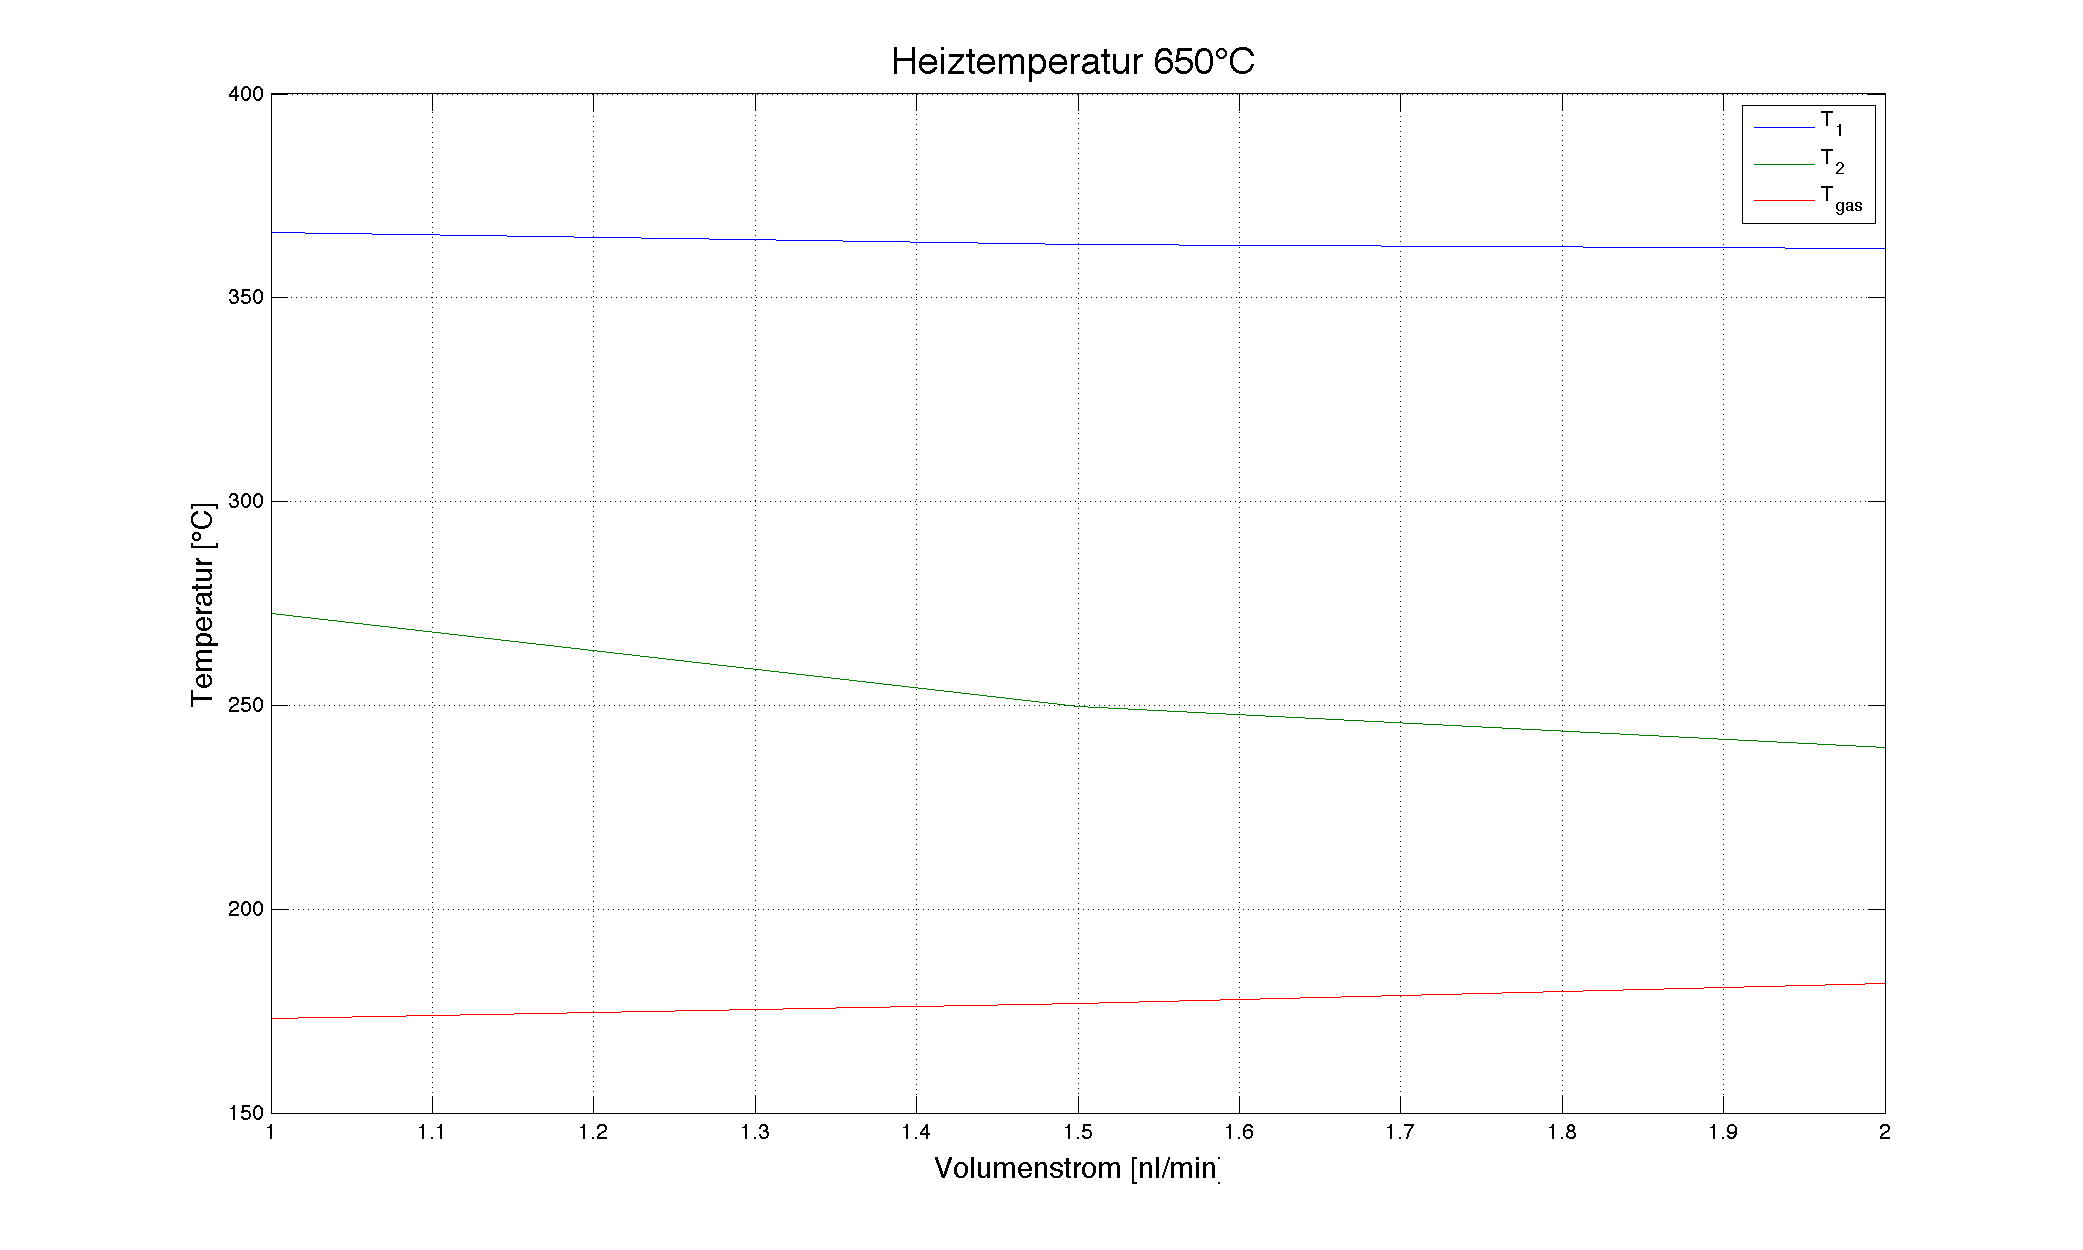
\includegraphics[width=\textwidth]{pics/figure1.png}
\caption{Messresultate}
\label{pic:figure1}
\end{figure}


